% !TEX root = domain_transduction.tex
We evaluate our algorithm on various unsupervised domain adaptation tasks while focusing on two different problems, hand-written digit classification and object recognition. For each experiment, we use three domains and extensively evaluate all transfer scenarios.

\subsection{Dataset}
In order to experiment our algorithm on the task of digit classification, we use MNIST\cite{mnist}, Street View House Number\cite{svhn} and artificailly generated version of MNIST, MNIST-M\cite{ganin15}. MNIST is the collection of 60k handwritten digits. For MNIST-M, we generate a series of digit images by using the original MNIST dataset and the color images of BSDS500\cite{bsds500} following the method explained in \cite{ganin15}. Since the dataset is not distributed directly by the authors, we further confirmed that the performance is similar to experimented in \cite{ganin15}. Street view house numbers dataset is a collection of house numbers collected directly from Google street view images. Among many important differences exist between these domains, most significant ones are MNIST being grayscale and the others being colored, SVHN images having extra confusing digits around the centered digit of interest. Moreover, all three of these domains are large-scale having at least 60k examples over 10 classes. 

On the other hand, we use Office\cite{office} dataset in order to evaluate our algorithm on the task of object recognition. Office dataset includes images of the same objects taken directly from Amazon, captured with a cheap webcam and captured with a D-SLR camera. Notable differences of these domains include the white background of Amazon images vs realistic backgrounds of webcam and D-SLR images, and the resolution difference of webcam and D-SLR. Office dataset have rather fewer number of images as maximum 2478 images per domain. On the other hand, it has larger number of classes since there are 31 object categories.

\subsection{Implementation Details}
Although our algorithm have very few design parameters and we decide most of them either using cross-validation or exhaustive grid search, our algorithm uses an existing differentiable feature function. The selection of this feature function is a critical parameter for our algorithm. Following the unparalleled success of convolutional neural networks (CNNs), we use CNNs as our feature functions.  In order to have  fair comparison with existing algorithms, we follow the same architecture used by \cite{ganin15}. We only change the feature dimensionality and experiment on the effect of feature dimension. Hence, we use the following architectures for domains \emph{(see supplementary material for full details)}:

\noindent \textbf{MNIST, MNIST-M} and \textbf{SVHN:} Modified LeNet\cite{lenet} as;

\includegraphics[width=\columnwidth]{lenet}


\noindent \textbf{Office:} Modified AlexNet\cite{alexnet} as;

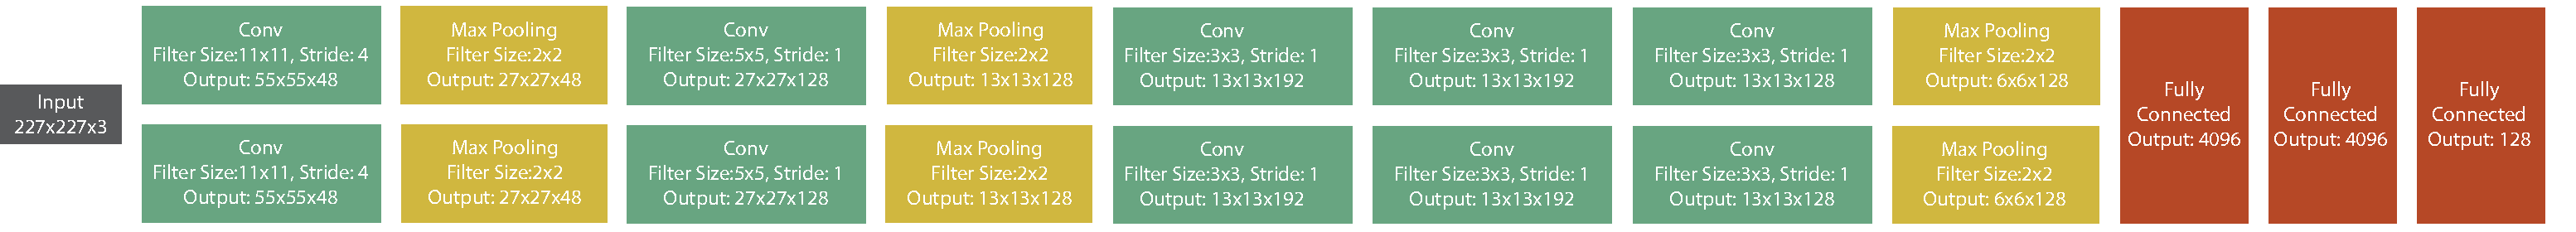
\includegraphics[width=\columnwidth]{alexnet}


where \textbf{C} is convolution, \textbf{P} is max-pooling, \textbf{R} is ReLU and \textbf{F} is fully connected layer. 

Since the office dataset is quite small, we do not learn the full network for office experiments instead we only optimize for fully connected layers initializing with the weights  pre-trained on ImageNet. Moreover, in all of our experiments we set the feature dimension as $128$. We use stochastic gradient descent in order to learn the feature function as well as the similarity metric with AdaGrad\cite{adagrad}. We initialize all variables with truncated normals having unit variance and use the learning rate $2.5x10^{-4}$ and the batch size $256$. 



We further share our learned models as well as the source code using TensorFlow\cite{tensorflow} on \url{http://anonymous.xyz}


\subsection{Evaluation Procedure}
We are evaluating all of the algorithms using the \emph{fully-transductive} setting. In other words,  we feed training set of source and target to our transductive domain adaptation algorithm. As an evaluation, we directly evaluate the labels obtain for the target unsupervised training data. We report the accuracy as the learning metric. Accuracy is the ratio of the correctly classified data points to the target unsupervised training data points.

\subsection{Results}
\begin{table*}[t]
\caption{Accuracy of our method and the state-of-the-art algorithms on Office dataset and various adaptation settings}
\label{tab:res}
\begin{sc}
\begin{center}
\begin{small}
\begin{tabular}{@{}rcccccc@{}} \toprule 
 Source & Amazon & D-SLR & Webcam & Webcam &Amazon & D-SLR \\
 Target & Webcam & Webcam & D-SLR & Amazon & D-SLR & Amazon \\
 \midrule
GFK \cite{gong2012} & $.398$ & $.791$ & $.746 $ & $.371$ & $.379$ & .379   \\
SA* \cite{fernando13} & $.450$ & $.648$ & $.699$ & $.393$ & $.388$ & $.420$ \\
DLID \cite{chopra13} & $.519$ & $.782$ & $.899$ & -&- &- \\
DDC \cite{tzeng14} & $.618$ & $.950$ & $.985$ & $.522$ & $.644$& $.521$\\
DAN \cite{wang15} & $.685$ & $.960$ & $.990$ & $.531$ & $.670$ & $.540$ \\
Backprop \cite{ganin15} & $.730$ &$\mathbf{.964}$ & $\mathbf{.992}$ & $.536$ & $.728$ & $.544$\\
\midrule
Source Only & $.642$ & $.961$ & $.978$ & $.452$ & $.668$ & $.476$ \\
Our Method & $\mathbf{.804}$ &.962 & $.989$ & $\mathbf{.625}$ & $\mathbf{.839}$ & $\mathbf{.567}$ \\
 \bottomrule
\end{tabular}
\end{small}
\end{center}
\end{sc}
\end{table*}



\begin{table}[t]
\caption{Accuracy of our method and the digit classification task.}
\label{tab:res}
\begin{sc}
\begin{small}
\resizebox{\columnwidth}{!}{%
\begin{tabular}{@{}r@{\hskip 1mm}c@{\hskip 1mm}c@{\hskip 1mm}c@{\hskip 1mm}c@{}} \toprule 
Source & M-M & MNIST  & SVHN & MNIST \\
Target&  MNIST & M-M & MNIST & SVHN\\
 \midrule
SA* \cite{fernando13}&  & $.569$ & $.593$ & \\
BP \cite{ganin15} &$.732$ & $.766$ & $.738$ & $.289$ \\
\midrule
Source Only  & $.483$ & $.522$  &.549 &\\
Our Method & $\mathbf{.835}$ & $\mathbf{.855}$ & $\mathbf{.774}$ & $\mathbf{.323}$\\
 \bottomrule
\end{tabular}}
\end{small}
\end{sc}
\end{table}

We compare our method with all state-of-the-art unsupervised domain adaptation algorithms and summarize the results in Table~\ref{tab:res}. 

Table~\ref{tab:res} suggests that our algorithm is on-par/slightky with state of the art method for D-SLR$\leftrightarrow$Webcam experiments. This is rather expected since the domain difference is very minor between D-SLR and webcam images. Considering the fact that we are using nearest neighbor as a classifier, our algorithm needs large-dataset to be successful. Both webcam and D-SLR datasets are rather small (300to700 examples) which limits the accuracy of nearest neighbor algorithm.

Table~\ref{tab:res} suggests our algorithm significantly outperforms all other examples when there is large domain difference like MNIST$\leftrightarrow$MNIST-M, Amazon$\leftrightarrow$Webcam and Amazon$\leftrightarrow$D-SLR. We believe this results is mostly due to the transductive modeling. All competing algorithms are seeking for features and models independent of domains, in other words they seek of classifiers which will be accurate on all domains. However, this is rather counter-intuitive when there is large domain difference like Amazon images vs webcam images or textured images vs handwritten digits. We seek for asymmetric transformation between domains. In other words, instead of invariance, we seek for equivariance. 


\subsubsection{Effect of label propagation and feature learning}
In order to evaluate the effect of having a robust label propagation and feature learning, we compare our method with a variant without the label propagation (noted as \emph{our-method-no-prop}) and a variant without feature learning (noted as \emph{our-method-no-fl}). We plot the accuracy vs number of iterations in order to evaluate both the effect on learning rate as well as the resultant accuracy. Although we plot the results only for MNIST$\rightarrow$MNIST-M, the other experiments have similar results and not displayed for the sake of clarity. Results are show in the Figure~\ref{fllprop}. 

As the Figure~\ref{fllprop} suggests, both feature learning and label propagation is crucial for successful transduction. The feature learning has a slightly larger effect. Moreover the necessity of domain invariant features are proven to be helpful in various work\cite{ganin15, tzeng14} in the literature. We further analyze the learned features as well as the label propagation performance more qualitatively in the following sections.

\begin{figure}[ht]
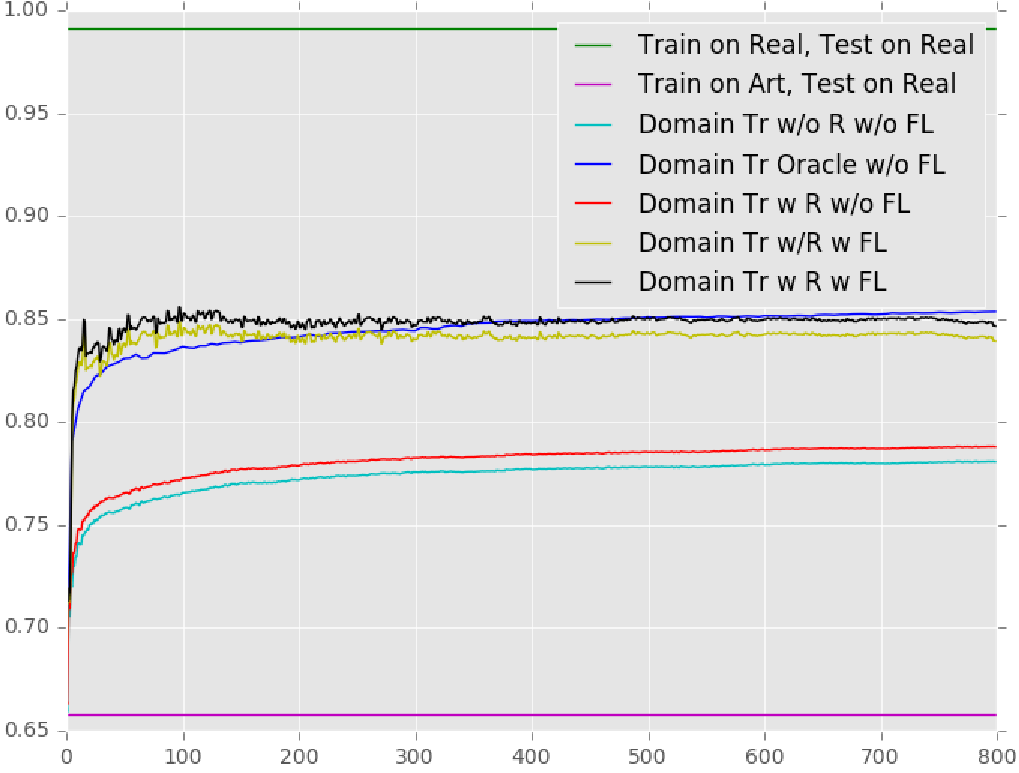
\includegraphics[width=\columnwidth]{figure_1fl}
\caption{Accuracy vs number of iterations for our-method, our-method-no-prop and our-method-no-fl. As the figure suggests the label propagation both increase the learning rate as well as the final accuracy. Moreover, the feature learning also have a significant effect on the accuracy.}
\label{fllprop}
\end{figure}

\subsubsection{Qualitative Analysis}

\begin{figure*}[ht]
    \begin{subfigure}[b]{0.5\textwidth}
        \includegraphics[width=\textwidth]{na_st.png}
        \caption{S. and T. w/o Adaptation}
        \label{fig:gull}
    \end{subfigure}~\begin{subfigure}[b]{0.5\textwidth}
        \includegraphics[width=\textwidth]{st.png}
        \caption{S. and T. with Adaptation}
        \label{fig:gull}
    \end{subfigure}

    \begin{subfigure}[b]{0.5\textwidth}
        \includegraphics[width=\textwidth]{sc.png}
        \caption{Source Labels w/ Adaptation}
        \label{fig:gull}
    \end{subfigure}~\begin{subfigure}[b]{0.5\textwidth}
        \includegraphics[width=\textwidth]{tc.png}
        \caption{Target Labels w/ Adaptation}
        \label{fig:gull}
    \end{subfigure}
\caption{tSNE plots for features without and with unsupervised adaptation. Please note that the discriminative behavior emerges in the unsupervised target instead of source domain. This explain the motivation behind modeling the problem as transduction. In other words, our algorithm is designed to be accurate and discriminative in the target domain which is the domain we are interested in. Also note that our features are not invariant but the nearest neighbor arrows suggests that there is a consistent transformation, in other words our features are equivariant. }
\end{figure*}


Here we will have t-SNE plots and some NN results

